\documentclass[border=3pt,tikz]{standalone}
\usepackage{tikz}
\usepackage{amsmath} % for \text
\usepackage{mathrsfs} % for \mathscr -> scri
\usepackage{xfp} % for fpeval -> floating point expression

\begin{document}
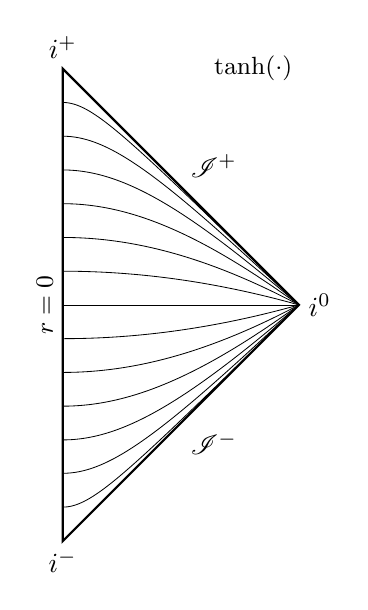
\begin{tikzpicture}[scale=3]
        
    % BOUNDING DIAGRAM
    \coordinate (O) at ( 0, 0); % center: origin (r,t) = (0,0)
    \coordinate (S) at ( 0,-1); % south: t=-infty, i-
    \coordinate (N) at ( 0, 1); % north: t=+infty, i+
    \coordinate (E) at ( 1, 0); % east:  r=+infty, i0
    \draw[thick] (N) -- (E) -- (S) -- cycle;
    
    % LABELS
    \newcommand{\scri}{\mathscr{I}} % null infinity
    \node[right] at (0.6,1) {\small{$\tanh(\cdot)$}};
    \node[right] at (E) {$i^0$};
    \node[above] at (N) {$i^+$};
    \node[below] at (S) {$i^-$};
    \node[above, rotate=90] at (O) {\small{$r=0$}};
    \node[above right] at (0.5,0.5) {$\scri^+$};
    \node[below right] at (0.5,-0.5) {$\scri^-$};
    
    % COMPACTIFICATION
    \newcommand\tanhe[1]{ (-1+exp(2*#1))/(1+exp(2*#1)) } % tanh in exp because tikz doesn't have it
    \tikzset{declare function={
        T(\t,\r)  = \fpeval{0.5*(\tanhe{\t+\r} + \tanhe{\t-\r})};
        R(\t,\r)  = \fpeval{0.5*(\tanhe{\t+\r} - \tanhe{\t-\r})};
    }}
    
    % FOLIATION
    \message{Drawing time surfaces.^^J}
    \def\Nlines{6} % total number of lines is 2\Nlines+1
    \newcommand\samp[1]{ 0.5*ln( (1+#1)/(1-#1)) } % equidistant sampling with inverse of compactifier
    \foreach \i [evaluate={\t=\i/(\Nlines+1);}] in {-\Nlines,...,\Nlines}{
        \message{Drawing i=\i...^^J}
        \draw[line width=0.3,samples=30,smooth,variable=\r,domain=0.001:1]
        plot({ R(\samp{\t},2*\samp{\r}) }, { T(\samp{\t},2*\samp{\r}) });
    }
    
\end{tikzpicture}
\end{document}